\begin{frame}{$n \pi^+ \pi-$不変質量による選別}
  \begin{tabular}{cc}
    \begin{minipage}{0.5\hsize}
      \scriptsize
      \textcolor{red}{$n \pi^+ \pi^-$不変質量 $>$1.7 $[GeV/c^2]$}\\
      $n \pi^+ \pi^-$不変質量 $<$1.7 $[GeV/c^2]$
    \end{minipage}

    \begin{minipage}{0.5\hsize}
      \begin{figure}
        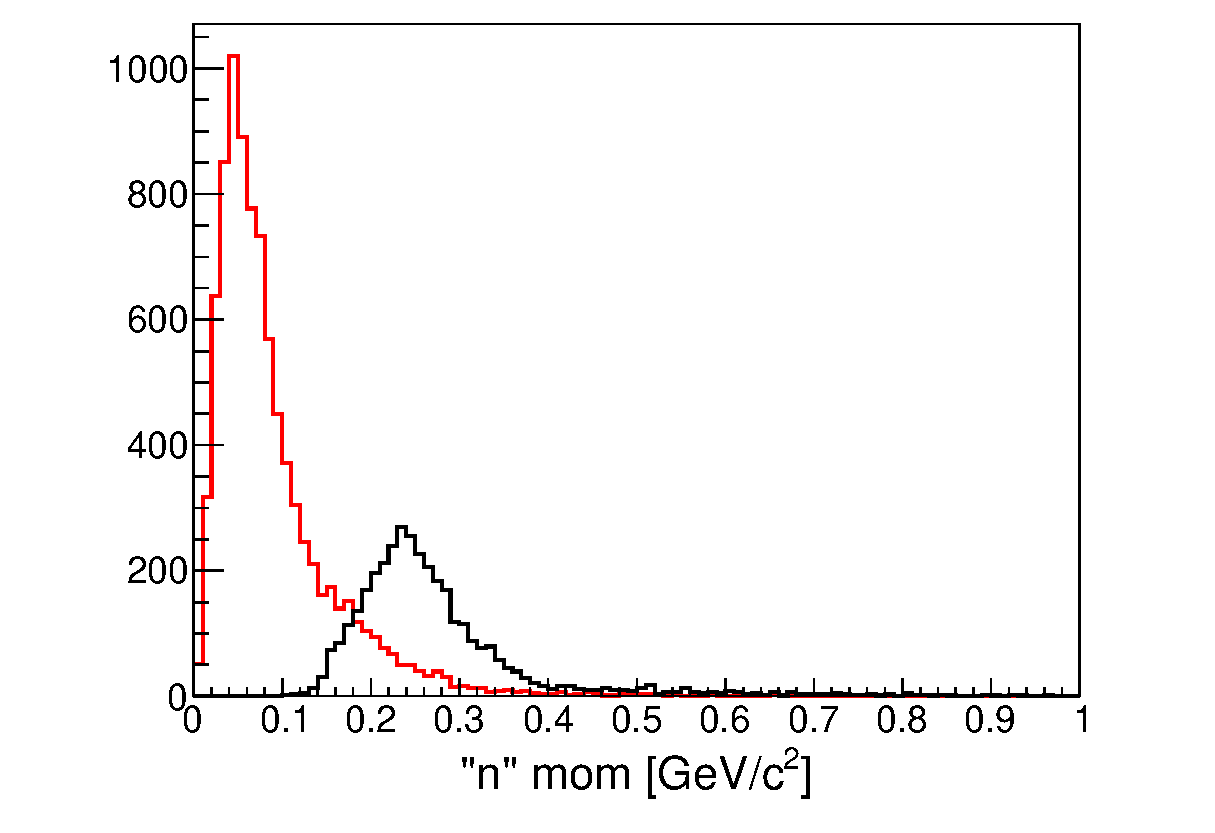
\includegraphics[width=5cm]{../pic/Run78/KN_ana/mmN_mom_p_select_K0.eps}
      \end{figure}
    \end{minipage}
  \end{tabular}

  \begin{tabular}{cc}
    \begin{minipage}{0.5\hsize}
      \begin{figure}
        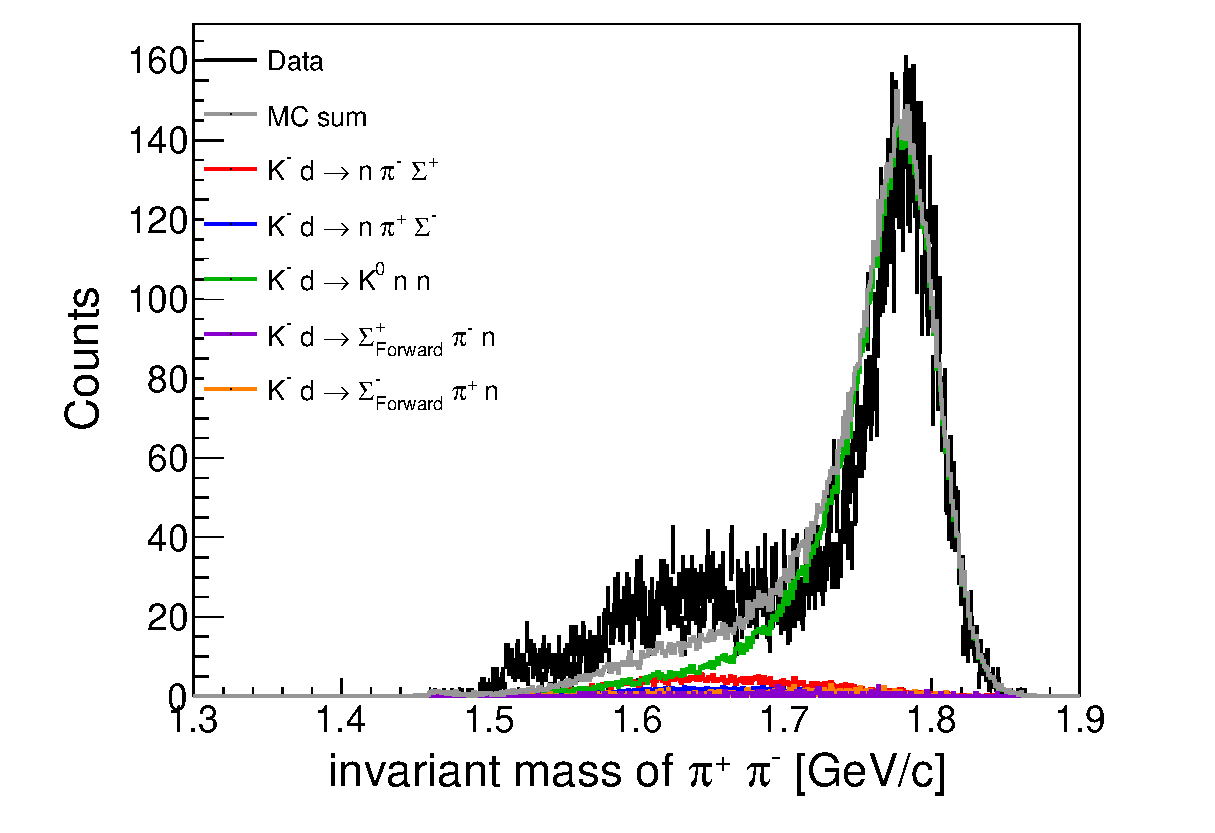
\includegraphics[width=5cm]{../pic/Run78/KN_ana/IM_npipi_K0.eps}
      \end{figure}
    \end{minipage}
    \begin{minipage}{0.5\hsize}
      \begin{figure}
        \includegraphics[width=5cm]{../pic/Run78/KN_ana/mmN_mom_IM_npipi_K0.eps}
      \end{figure}
    \end{minipage}
  \end{tabular}
  \centering
  $n \pi^+ \pi^-$不変質量が1.7$[GeV/c^2]$以上は1-step反応 
\end{frame}
